\documentclass[12pt,letterpaper]{article}
\usepackage{graphicx,textcomp}
\usepackage{natbib}
\usepackage{setspace}
\usepackage{fullpage}
\usepackage{color}
\usepackage[reqno]{amsmath}
\usepackage{amsthm}
\usepackage{fancyvrb}
\usepackage{amssymb,enumerate}
\usepackage[all]{xy}
\usepackage{endnotes}
\usepackage{lscape}
\newtheorem{com}{Comment}
\usepackage{float}
\usepackage{hyperref}
\newtheorem{lem} {Lemma}
\newtheorem{prop}{Proposition}
\newtheorem{thm}{Theorem}
\newtheorem{defn}{Definition}
\newtheorem{cor}{Corollary}
\newtheorem{obs}{Observation}
\usepackage[compact]{titlesec}
\usepackage{dcolumn}
\usepackage{tikz}
\usetikzlibrary{arrows}
\usepackage{multirow}
\usepackage{xcolor}
\newcolumntype{.}{D{.}{.}{-1}}
\newcolumntype{d}[1]{D{.}{.}{#1}}
\definecolor{light-gray}{gray}{0.65}
\usepackage{url}
\usepackage{listings}
\usepackage{color}

\definecolor{codegreen}{rgb}{0,0.6,0}
\definecolor{codegray}{rgb}{0.5,0.5,0.5}
\definecolor{codepurple}{rgb}{0.58,0,0.82}
\definecolor{backcolour}{rgb}{0.95,0.95,0.92}

\lstdefinestyle{mystyle}{
	backgroundcolor=\color{backcolour},   
	commentstyle=\color{codegreen},
	keywordstyle=\color{magenta},
	numberstyle=\tiny\color{codegray},
	stringstyle=\color{codepurple},
	basicstyle=\footnotesize,
	breakatwhitespace=false,         
	breaklines=true,                 
	captionpos=b,                    
	keepspaces=true,                 
	numbers=left,                    
	numbersep=5pt,                  
	showspaces=false,                
	showstringspaces=false,
	showtabs=false,                  
	tabsize=2
}
\lstset{style=mystyle}
\newcommand{\Sref}[1]{Section~\ref{#1}}
\newtheorem{hyp}{Hypothesis}

\title{Problem Set 3}
\date{November 11, 2024}
\author{Rafaela Alves}


\begin{document}
	\maketitle

\section*{Question 1}
\vspace{.25cm}
\noindent We are interested in knowing how the difference in campaign spending between incumbent and challenger affects the incumbent's vote share. 
	\begin{enumerate}
		
		
		\item Run a regression where the outcome variable is \texttt{voteshare} and the explanatory variable is \texttt{difflog}.	
				\vspace{.25cm}
				\lstinputlisting[language=R, firstline=46, lastline=47]{PS3_my_answers.R}  
				\begin{verbatim}
				Call:
				lm(formula = voteshare ~ difflog, data = inc.sub)
				
				Residuals:
				Min       1Q   Median       3Q      Max 
				-0.26832 -0.05345 -0.00377  0.04780  0.32749 
				
				Coefficients:
				Estimate Std. Error t value Pr(>|t|)    
				(Intercept) 0.579031   0.002251  257.19   <2e-16 ***
				difflog     0.041666   0.000968   43.04   <2e-16 ***
				---
				Signif. codes:  0 ‘***’ 0.001 ‘**’ 0.01 ‘*’ 0.05 ‘.’ 0.1 ‘ ’ 1
				
				Residual standard error: 0.07867 on 3191 degrees of freedom
				Multiple R-squared:  0.3673,	Adjusted R-squared:  0.3671 
				F-statistic:  1853 on 1 and 3191 DF,  p-value: < 2.2e-16
			\end{verbatim}
		
		
		\newpage
		
		
		\item Make a scatterplot of the two variables and add the regression line. 	
				\begin{figure}[h!]
				\centering
				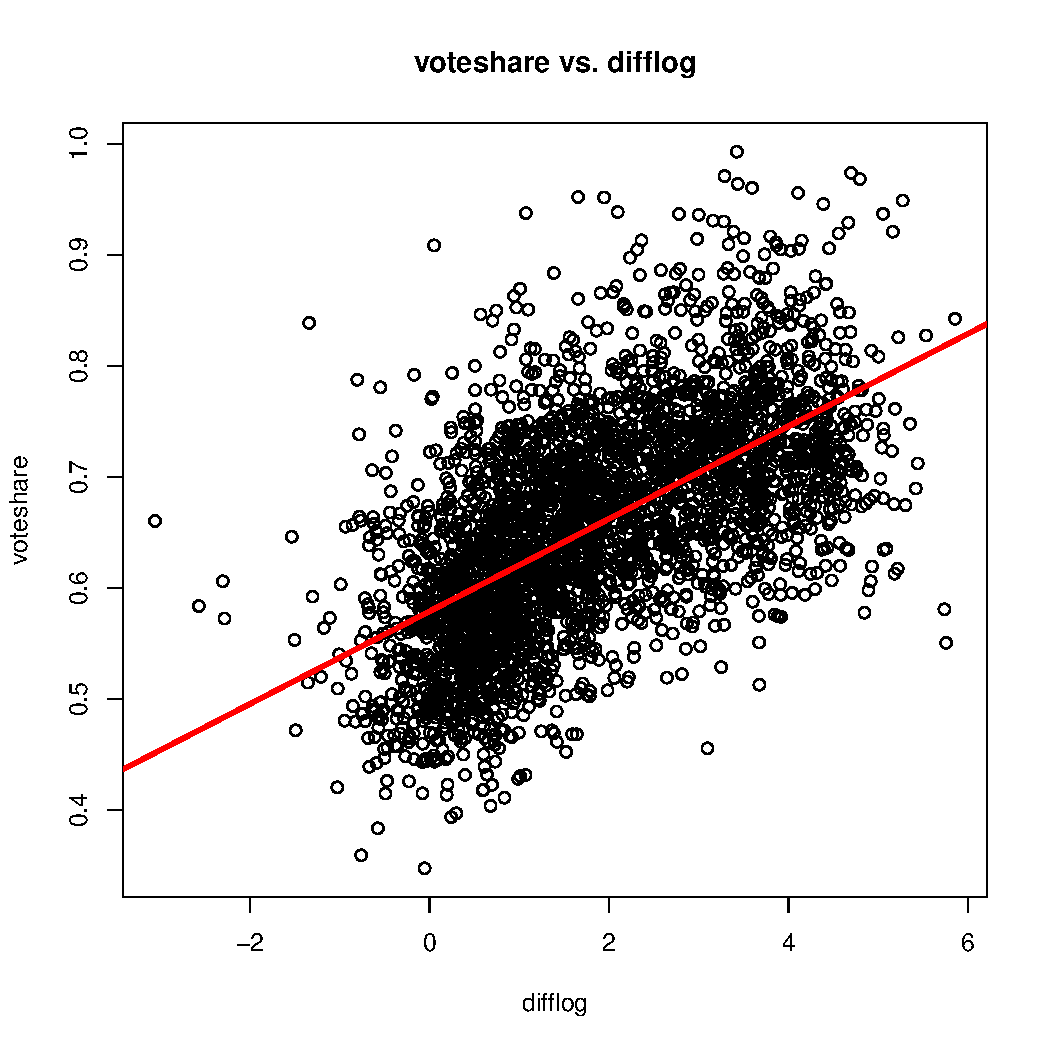
\includegraphics[width=0.55\textwidth]{plot_question1.pdf}
				\end{figure}
				\vspace{.4cm}
			
			
		\item Save the residuals of the model in a separate object.	
				\vspace{.25cm}
				\lstinputlisting[language=R, firstline=61, lastline=62]{PS3_my_answers.R} 
				\begin{verbatim}
				    1           2            3          4           5           6 
				-0.00042    -0.03168    -0.00455     0.03866     0.03552     0.03228 
				\end{verbatim}
				\vspace{.4cm}
		
		
		\item Write the prediction equation.
				\vspace{.25cm}
				\[
				\boldmath
				voteshare = 0.579 + 0.041 * difflog
				\]
				For every one-unit increase in difflog, the predicted voteshare increases by approximately 0.041 units. The starting point for voteshare is 0.579 when difflog is zero.
				\vspace{.25cm}
				\lstinputlisting[language=R, firstline=66, lastline=66]{PS3_my_answers.R} 
				\begin{verbatim}
				(Intercept)     difflog 
				0.57903071  0.04166632 
				\end{verbatim}			
			
	\end{enumerate}
	
\newpage

\section*{Question 2}
\noindent We are interested in knowing how the difference between incumbent and challenger's spending and the vote share of the presidential candidate of the incumbent's party are related.	\vspace{.25cm}
	\begin{enumerate}
	
	
		\item Run a regression where the outcome variable is \texttt{presvote} and the explanatory variable is \texttt{difflog}.	
			\vspace{.25cm}
			\lstinputlisting[language=R, firstline=80, lastline=81]{PS3_my_answers.R}  
			\begin{verbatim}
			Call:
			lm(formula = presvote ~ difflog, data = inc.sub)
			
			Residuals:
			Min       1Q   Median       3Q      Max 
			-0.32196 -0.07407 -0.00102  0.07151  0.42743 
			
			Coefficients:
			Estimate Std. Error t value Pr(>|t|)    
			(Intercept) 0.507583   0.003161  160.60   <2e-16 ***
			difflog     0.023837   0.001359   17.54   <2e-16 ***
			---
			Signif. codes:  0 ‘***’ 0.001 ‘**’ 0.01 ‘*’ 0.05 ‘.’ 0.1 ‘ ’ 1
			
			Residual standard error: 0.1104 on 3191 degrees of freedom
			Multiple R-squared:  0.08795,	Adjusted R-squared:  0.08767 
			F-statistic: 307.7 on 1 and 3191 DF,  p-value: < 2.2e-16
		\end{verbatim}
		\vspace{2cm}
	
		
		
		\item Make a scatterplot of the two variables and add the regression line. 	\vspace{5cm}
			\begin{figure}[h!]
			\centering
			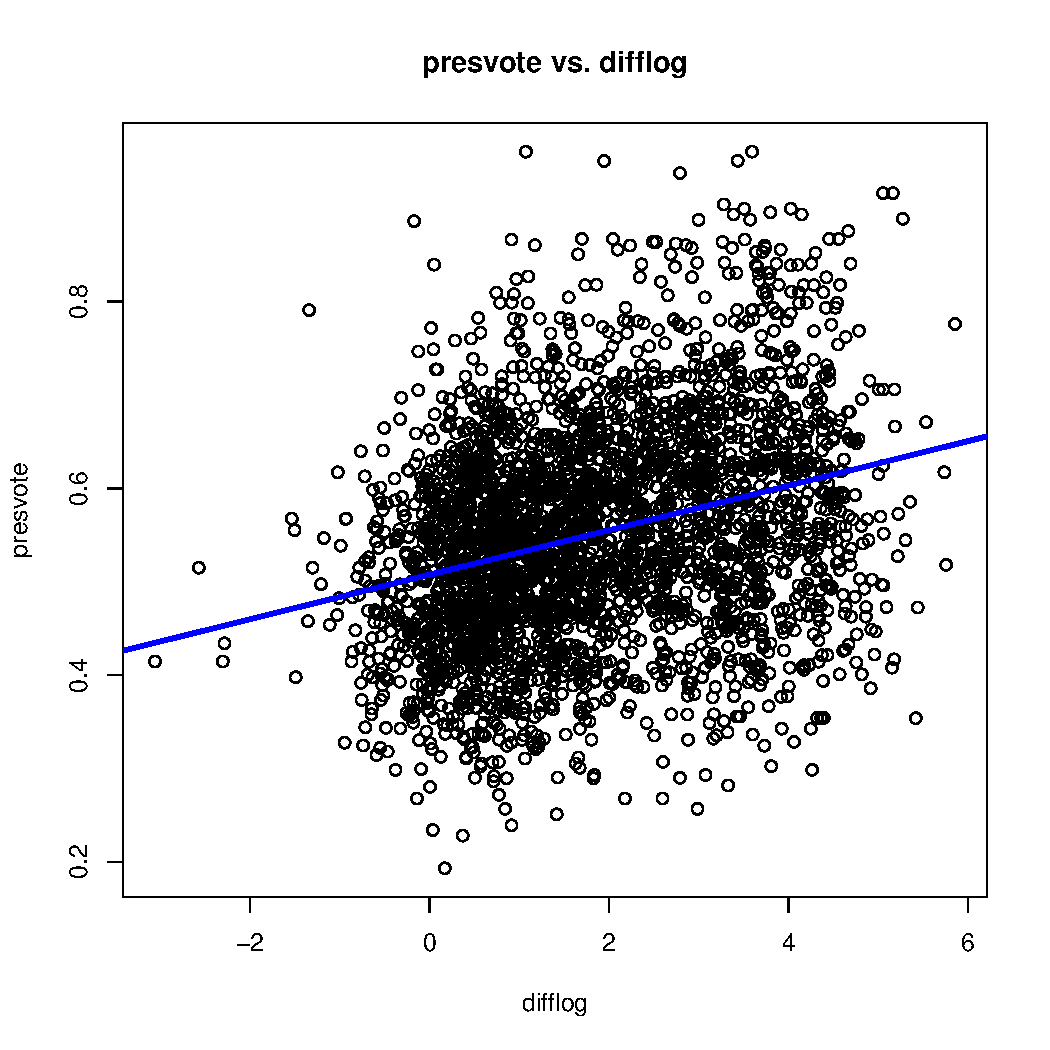
\includegraphics[width=0.55\textwidth]{plot_question2.pdf}
			\end{figure}
			\vspace{.5cm}
		
		
		
		\item Save the residuals of the model in a separate object.
			\vspace{.25cm}
			\lstinputlisting[language=R, firstline=95, lastline=96]{PS3_my_answers.R} 
			\begin{verbatim}
		  	 1            2            3         4           5            6 
			0.00560    0.03757     -0.05313     -0.05299    -0.04584    0.07433 
			\end{verbatim}
			\vspace{.5cm}
		
		
		\item Write the prediction equation.
			\vspace{.25cm}
			\[
			\boldmath
			\textbf
			presvote = 0.507 + 0.023 * difflog
			\]
			For every one-unit increase in difflog, the predicted presvote increases by approximately 0.023 units. The starting point for presvote when difflog is zero is around 0.507.
			\vspace{.25cm}
			\lstinputlisting[language=R, firstline=100, lastline=100]{PS3_my_answers.R} 
			\begin{verbatim}
			(Intercept)     difflog 
			0.50758333  0.02383723 
			\end{verbatim}			
		


	\end{enumerate}
	
	\newpage	
	
	

	
	
\section*{Question 3}

\noindent We are interested in knowing how the vote share of the presidential candidate of the incumbent's party is associated with the incumbent's electoral success.
	\vspace{.25cm}
	\begin{enumerate}
	
	
	
		\item Run a regression where the outcome variable is \texttt{voteshare} and the explanatory variable is \texttt{presvote}.
			\vspace{.25cm}
			\lstinputlisting[language=R, firstline=112, lastline=113]{PS3_my_answers.R}  
			\begin{verbatim}
			Call:
			lm(formula = voteshare ~ presvote, data = inc.sub)
			
			Residuals:
			Min       1Q   Median       3Q      Max 
			-0.27330 -0.05888  0.00394  0.06148  0.41365 
			
			Coefficients:
			Estimate Std. Error t value Pr(>|t|)    
			(Intercept) 0.441330   0.007599   58.08   <2e-16 ***
			presvote    0.388018   0.013493   28.76   <2e-16 ***
			---
			Signif. codes:  0 ‘***’ 0.001 ‘**’ 0.01 ‘*’ 0.05 ‘.’ 0.1 ‘ ’ 1
			
			Residual standard error: 0.08815 on 3191 degrees of freedom
			Multiple R-squared:  0.2058,	Adjusted R-squared:  0.2056 
			F-statistic:   827 on 1 and 3191 DF,  p-value: < 2.2e-16
			\end{verbatim}
			\vspace{2cm}
	
	
				\newpage	
	
	
		\item Make a scatterplot of the two variables and add the regression line. 
				\begin{figure}[h!]
				\centering
				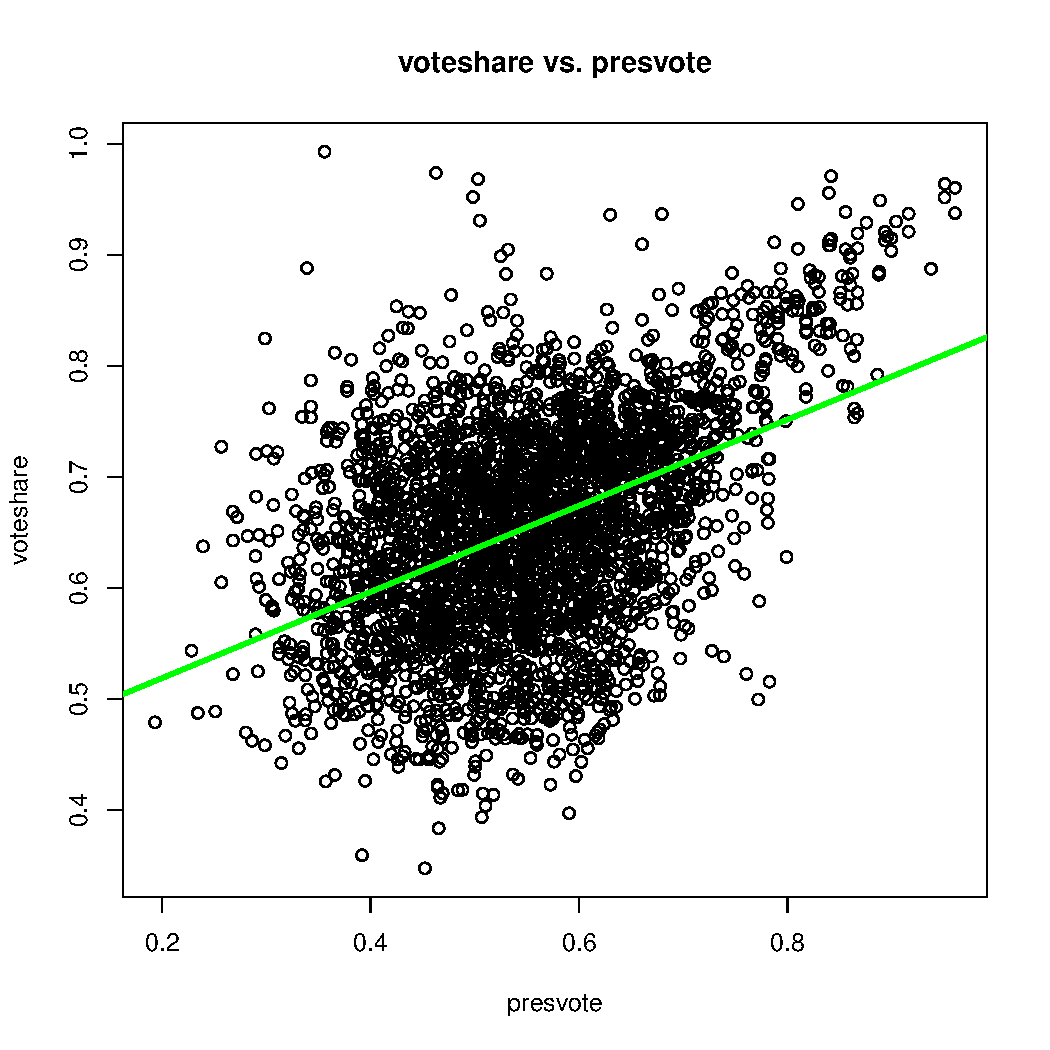
\includegraphics[width=0.55\textwidth]{plot_question3.pdf}
				\end{figure}
				\vspace{1cm}
	
	
	
	
		\item Write the prediction equation.
			\vspace{.25cm}
			\[
			\boldmath
			\textbf
			voteshare = 0.441 + 0.388 * presvote
			\]
			For every one-unit increase in presvote, the predicted voteshare increases by approximately 0.388 units. The starting point for voteshare when presvote is zero is around 0.441.
			\vspace{.25cm}
			\lstinputlisting[language=R, firstline=127, lastline=127]{PS3_my_answers.R} 
			\begin{verbatim}
			(Intercept)    presvote 
			0.4413299   0.3880184 
			\end{verbatim}			
		
	
	\end{enumerate}
	
	
	
	
\newpage	



\section*{Question 4}
\noindent The residuals from part (a) tell us how much of the variation in \texttt{voteshare} is $not$ explained by the difference in spending between incumbent and challenger. The residuals in part (b) tell us how much of the variation in \texttt{presvote} is $not$ explained by the difference in spending between incumbent and challenger in the district.
	\begin{enumerate}
		\vspace{.5cm}
		
		
		\item Run a regression where the outcome variable is the residuals from Question 1 and the explanatory variable is the residuals from Question 2.
			\vspace{.5cm}
			
			Y outcome = {residuals\_model1}
			
			X predictor = {residuals\_model2}
			\vspace{.5cm}
			
		\lstinputlisting[language=R, firstline=143, lastline=144]{PS3_my_answers.R}  
		\begin{verbatim}
		Call:
		lm(formula = residuals_model1 ~ residuals_model2)
		
		Residuals:
		Min       1Q   Median       3Q      Max 
		-0.25928 -0.04737 -0.00121  0.04618  0.33126 
		
		Coefficients:
		Estimate Std. Error t value Pr(>|t|)    
		(Intercept)      -5.934e-18  1.299e-03    0.00        1    
		residuals_model2  2.569e-01  1.176e-02   21.84   <2e-16 ***
		---
		Signif. codes:  0 ‘***’ 0.001 ‘**’ 0.01 ‘*’ 0.05 ‘.’ 0.1 ‘ ’ 1
		
		Residual standard error: 0.07338 on 3191 degrees of freedom
		Multiple R-squared:   0.13,	Adjusted R-squared:  0.1298 
		F-statistic:   477 on 1 and 3191 DF,  p-value: < 2.2e-16
		\end{verbatim}
		\vspace{2cm}
		
		
		
		\newpage	
		
		

		\item Make a scatterplot of the two residuals and add the regression line.
			\begin{figure}[h!]
			\centering
			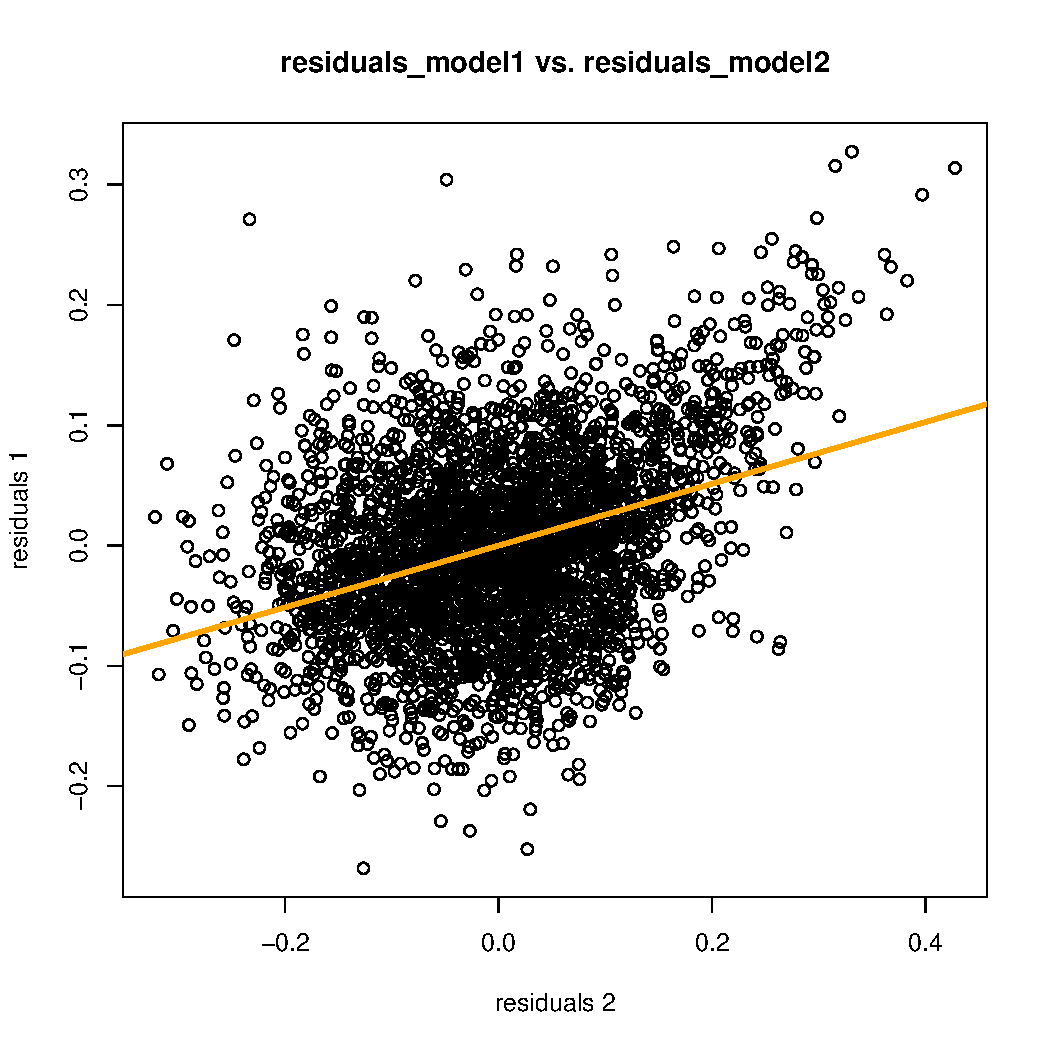
\includegraphics[width=0.55\textwidth]{plot_question4.pdf}
			\end{figure}
			\vspace{1cm}
		
		

		
		\item Write the prediction equation.
			\vspace{.25cm}
			\[
			\boldmath
			\textbf
			residuals\_model1 = -5.934 + 2.568 * residuals\_model2
			\]
			For each unit increase in the residuals\_model2, the residuals\_model1 increase by approximately 2.568 units. The starting point for residuals\_model1 is negative, -5.934, when residuals\_model2 is zero.
			\vspace{.25cm}
			\lstinputlisting[language=R, firstline=158, lastline=158]{PS3_my_answers.R} 
			\begin{verbatim}
			 (Intercept)      residuals_model2 
			-5.934078e-18     2.568770e-01 
			\end{verbatim}			
		
		
		
	\end{enumerate}
	
	\newpage	

\section*{Question 5}
\noindent What if the incumbent's vote share is affected by both the president's popularity and the difference in spending between incumbent and challenger? 
	\begin{enumerate}
	
	
		\item Run a regression where the outcome variable is the incumbent's \texttt{voteshare} and the explanatory variables are \texttt{difflog} and \texttt{presvote}.	
			\vspace{.5cm}
		
			Y = voteshare
		
			X1 = difflog (campaing spending)
			
			X2 = presvote (president’s popularity)
			\vspace{.5cm}
		
			\lstinputlisting[language=R, firstline=176, lastline=177]{PS3_my_answers.R}  
			\begin{verbatim}
			Call:
			lm(formula = voteshare ~ difflog + presvote, data = inc.sub)
		
			Residuals:
			Min       1Q   Median       3Q      Max 
			-0.25928 -0.04737 -0.00121  0.04618  0.33126 
		
			Coefficients:
			Estimate Std. Error t value Pr(>|t|)    
			(Intercept) 0.4486442  0.0063297   70.88   <2e-16 ***
			difflog     0.0355431  0.0009455   37.59   <2e-16 ***
			presvote    0.2568770  0.0117637   21.84   <2e-16 ***
			---
			Signif. codes:  0 ‘***’ 0.001 ‘**’ 0.01 ‘*’ 0.05 ‘.’ 0.1 ‘ ’ 1
		
			Residual standard error: 0.07339 on 3190 degrees of freedom
			Multiple R-squared:  0.4496,	Adjusted R-squared:  0.4493 
			F-statistic:  1303 on 2 and 3190 DF,  p-value: < 2.2e-16
			\end{verbatim}



	\newpage	
		
		
		
		
		\item Write the prediction equation.
			\vspace{.25cm}
			\[
			\boldmath
			\textbf
			voteshare = 0.448 + 0.035 * difflog + 0.256 * presvote
			\]
			For each unit increase in difflog, the voteshare increases by approximately 0.035 units, assuming presvote remains constant. 
			For each unit increase in presvote, the voteshare increases by approximately 0.256 units, assuming difflog remains constant. 
			The starting point for voteshare is 0.448 when both, difflog and presvote are zero.
			\vspace{.25cm}
			\lstinputlisting[language=R, firstline=181, lastline=181]{PS3_my_answers.R} 
			\begin{verbatim}
			(Intercept)     difflog         presvote 
			0.44864422      0.03554309      0.25687701 
			\end{verbatim}			
		
		
		

		
		
		
		
		\item What is it in this output that is identical to the output in Question 4? Why do you think this is the case?
	\end{enumerate}
	\vspace{.50cm}

		The RESIDUALS in Question 4 are identical to the ones in Question5. 
		\vspace{.25cm}
		
		In the regression in Question 4, we're regressing the residuals from model1 (what remains in \textbf{voteshare} after accounting for \textbf{difflog}) and model2 (what remains in \textbf{presvote} after accounting for \textbf{difflog}). 
		It checks if there is a relationship between these two residuals, which corresponds to the part of \textbf{voteshare} explained by \textbf{presvote} after controlling for \textbf{difflog}.
		\vspace{.25cm}

		In Question 5 regression, we use \textbf{difflog} and \textbf{presvote} as predictors of \textbf{voteshare}. The residuals in this case are what remains in \textbf{voteshare} after accounting \textbf{difflog} and \textbf{presvote}. 
		\vspace{.25cm}
		
		Summarizing, both sets of residuals are showing the "unexplained" part of \textbf{voteshare} after accounting the effect of \textbf{difflog} and \textbf{presvote}.









\end{document}
